% !TeX program = txs:///arara
% arara: pdflatex: {synctex: on, interaction: nonstopmode, shell: yes}
\documentclass{article}
\usepackage[svgnames]{xcolor}
\usepackage{tikz}

\usepackage[paper=a3paper,landscape,paperwidth=60cm]{geometry}

\usepackage{bbding}

\newcommand{\duck}[1]{%

	\colorlet{duck}{#1}
	\colorlet{eye}{Cornsilk}
	\colorlet{pupil}{black}
	\colorlet{bill}{orange}
		
	%body
	\path[fill=duck] (51.2815,135.5394) .. controls (26.6859,139.7884) and (-12.5215,184.2616) .. (28.9411,223.8858) .. controls (70.4036,263.5099) and (286.2675,236.9673) .. (181.7701,108.1215) .. controls (93.7517,155.4266) and (123.9624,112.1537) .. (51.2815,135.5394) -- cycle;

	%head
	\path[fill=duck] (90,100) ellipse (1.4cm and 1.75cm);
	
	% duck's bill
	\path[fill=bill, xshift=-11pt, xscale=1.1] (49.3866,102.7929) .. controls (70.9472,97.0244) and (61.6632,119.6616) .. (95.1826,113) .. controls (20,165) and (36.9082,113.0997) .. (49.3866,102.7929) -- cycle;
	
	% right eye
	\path[fill=eye, rotate=20, xshift=-4pt, yshift=1pt] (112,58) ellipse (0.25cm and 0.35cm);
	\path[fill=pupil, rotate=20, xshift=-4pt, yshift=1pt] (115,59) ellipse (0.1cm and 0.2cm);
	
	% left eye
	\path[fill=eye, rotate=20] (78,62) ellipse (0.22cm and 0.32cm);
	\path[fill=pupil, rotate=20] (81,63) ellipse (0.08cm and 0.18cm);

}

\newcommand{\addalien}{%
	\draw[line width=3pt,color=YellowGreen] (110,62) -- (130,20);
	\draw[line width=3pt,color=YellowGreen] (72,58) -- (60,15);
	\path[fill=YellowGreen] (130,20) circle (0.2cm);
	\path[fill=YellowGreen] (60,15) circle (0.2cm);
}

\newcommand{\addhat}[1]{%
	\path[fill=#1] (90,55) ellipse (1.3cm and 0.25cm);
	\path[fill=#1] (90,30) ellipse (0.7cm and 0.2cm);
	\path[fill=#1] (115,30) rectangle (65,55);
}

\newcommand{\addsunglasses}{
	\draw[line width=3pt,color=black] (50,95) arc (190:370:20) ;
	\path[draw=black,line width=3pt] (100,90) -- (130,100);
	\path[fill=black, rotate=20] (116,56) ellipse (0.4cm and 0.4cm);
	\path[fill=black, rotate=20] (80,60) ellipse (0.37cm and 0.37cm);
}

\newcommand{\addicecream}[3]{
	\path[draw=Sienna,fill=Goldenrod,line width=1pt,yshift=50pt,rotate=20,xshift=50pt] 
	(45,60)--(60,120)--(75,60);
	\path[draw=Sienna, fill=Goldenrod, rotate=20,line width=1pt] (144,118) ellipse (0.4cm and 0.25cm);
	\path[fill=#1, rotate=20] (138,116) circle (0.3cm);
	\path[fill=#2, rotate=20] (148,116) circle (0.3cm);
	\path[fill=#3, rotate=20] (142,102) circle (0.3cm);
}

\newcommand{\addunicorn}{
	\path[draw=VioletRed,fill=Pink,line width=1pt,yshift=20pt,rotate=-25,xshift=0pt] 
	(50,60)--(60,20)--(70,60);
}

\newcommand{\addhair}[1]{%
	\path[fill=#1, xshift=-5pt] (151.3277,174.3473) .. controls (157.7099,171.1213) and (164.7938,167.8644) .. (168.7230,161.6896) .. controls (164.8427,161.5316) and (153.5102,155.4255) .. (162.1164,152.9395) .. controls (169.4207,153.1460) and (176.4092,149.5358) .. (179.3920,142.6587) .. controls (185.5577,133.4026) and (172.4051,138.2448) .. (169.0163,134.3455) .. controls (174.7801,132.5948) and (184.6532,131.7138) .. (187.4798,127.5635) .. controls (176.4675,125.1191) and (163.1258,123.3733) .. (156.8817,112.6068) .. controls (152.4387,98.5734) and (153.2098,83.5059) .. (149.6492,69.2411) .. controls (131.4926,-1.1678) and (29.6020,22.0627) .. (47.7294,90.0940) .. controls (49.6639,62.0732) and (72.5401,38.6998) .. (96.3583,54.2220) .. controls (130.5162,76.1752) and (139.7469,117.8581) .. (115.3043,143.8986) .. controls (115.2213,148.9109) and (117.2762,158.3403) .. (124.2981,163.2993) .. controls (131.3200,168.2584) and (141.2814,171.4676) .. (151.3277,174.3473) -- cycle;
}

\newcommand{\addshirt}[1]{%
	\path[fill=#1] (50,135.5394) .. controls (26.6859,139.7884) and (-12.5215,184.2616) .. (28.9411,223.8858) .. controls (70.4036,263.5099) and (286.2675,236.9673) .. (181.7701,108.1215) .. controls (93.7517,155.4266) and (123.9624,112.1537) .. (51.2815,180) -- cycle;
}

\newcommand{\addtie}[1]{
	\draw[line width=10pt,color=#1] (60,150) -- (50,190);
}

\newcommand{\addtshirt}[1]{
	\path[fill=#1] (50,135.5394) .. controls (26.6859,139.7884) and (-12.5215,184.2616) .. (28.9411,223.8858) .. controls (70.4036,263.5099) and (286.2675,236.9673) .. (181.7701,108.1215) .. controls (93.7517,155.4266) and (123.9624,122.1537) .. (59,150) -- cycle;
}

\newcommand{\addshorthair}[1]{
	\path[fill=#1, xshift=-5pt] (145.7190,108.2466) .. controls (151.7052,104.8240) and (153.2448,84.3447) .. (149.6842,70.0799) .. controls (131.5276,-0.3291) and (29.6371,22.9015) .. (47.7644,90.9328) .. controls (49.6989,62.9120) and (80.4610,40.0060) .. (101.1924,59.4599) .. controls (128.6626,85.2375) and (139.4074,111.8552) .. (145.7190,108.2466) -- cycle;
}

\newcommand{\addwizzard}{
	\path[fill=BlueViolet!50!Pink,line width=1pt,yshift=-40pt,rotate=5,xshift=32pt] 
	(20,100)--(60,0)--(100,100);
	\pgftext[at=\pgfpoint{71}{-15}, left, base]{\color{Gold}\EightStarBold}
	\pgftext[at=\pgfpoint{63}{0}, left, base]{\color{Gold}\EightStarBold~\EightStarBold}
	\pgftext[at=\pgfpoint{56}{15}, left, base]{\color{Gold}\EightStarBold~\EightStarBold~\EightStarBold}
	\pgftext[at=\pgfpoint{56}{30}, left, base]{\color{Gold}\EightStarBold~\EightStarBold~\EightStarBold}
	\draw[line width=6pt,color=black] (90,160) -- (60,210);
	\draw[line width=6pt,color=white] (85,168.333) -- (80,176.666);
}

\begin{document}

%%Christian Hupfer
%\begin{tikzpicture}[y=0.80pt, x=0.80pt, yscale=-1.000000, xscale=1.000000, inner sep=0pt, outer sep=0pt]
%	\duck{Gold}
%	\addwizzard
%\end{tikzpicture}
%%
%% short hairs
%\begin{tikzpicture}[y=0.80pt, x=0.80pt, yscale=-1.000000, xscale=1.000000, inner sep=0pt, outer sep=0pt]
%	\duck{Wheat}
%	\addtshirt{LightBlue!50!white}
%	\addshirt{LightSlateGrey}
%	\addshorthair{brown!50!Grey}
%\end{tikzpicture}
%%
%%Men in black
%\begin{tikzpicture}[y=0.80pt, x=0.80pt, yscale=-1.000000, xscale=1.000000, inner sep=0pt, outer sep=0pt]
%	\duck{Wheat}
%	\addtshirt{white}
%	\addshirt{black}
%	\addtie{black}
%	\addhat{black}
%	\addsunglasses
%\end{tikzpicture}
%%
%% swimming
%\begin{tikzpicture}[y=0.80pt, x=0.80pt, yscale=-1.000000, xscale=1.000000, inner sep=0pt, outer sep=0pt]
%	\duck{Gold}
%	\foreach \i in {1,...,100} {
%	   \pgfmathsetmacro{\x}{random(0,200)}%
%	   \pgfmathsetmacro{\y}{random(150,200)}%
%	   \pgftext[at=\pgfpoint{\x}{\y}, left, base]{\textcolor{blue!\i!black}{\rotatebox{90}{S}}}
%	}; 
%\end{tikzpicture}
%
%% ducklings
%\begin{tikzpicture}[y=0.80pt, x=0.80pt, yscale=-0.6, xscale=0.6, inner sep=0pt, outer sep=0pt]
%	\duck{Gold}
%	\begin{scope}[xshift=300pt, scale=.3, yshift=400pt]
%		\duck{Gold}
%	\end{scope}
%	\begin{scope}[xshift=180pt, scale=.3, yshift=350pt]
%		\duck{Gold}
%	\end{scope}
%	\begin{scope}[xshift=240pt, scale=.3, yshift=450pt]
%		\duck{Gold}
%	\end{scope}		
%\end{tikzpicture}
%
% samcarter
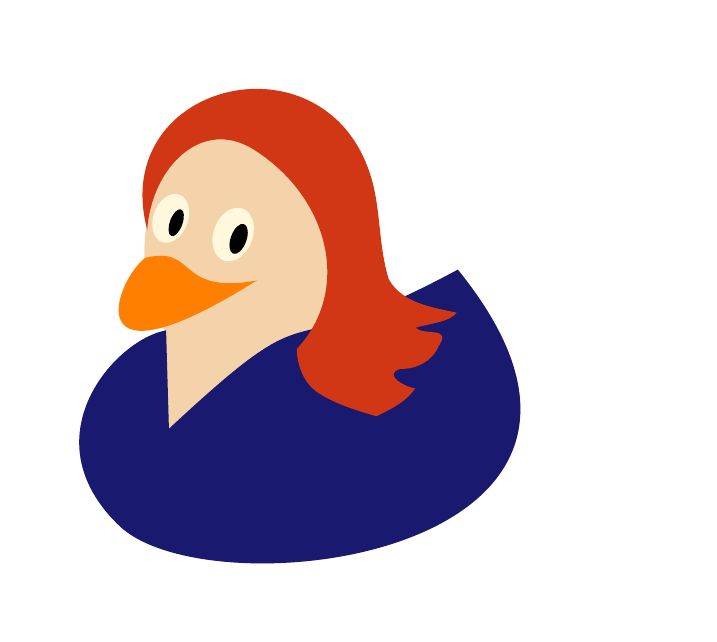
\begin{tikzpicture}[y=0.80pt, x=0.80pt, yscale=-1.000000, xscale=1.000000, inner sep=0pt, outer sep=0pt]
	\duck{Wheat!95!red}
	\addshirt{MidnightBlue}
	\addhair{OrangeRed!50!Brown}
\end{tikzpicture}
%
%% hair
%\begin{tikzpicture}[y=0.80pt, x=0.80pt, yscale=-1.000000, xscale=1.000000, inner sep=0pt, outer sep=0pt]
%	\duck{Gold}
%	\addhair{SeaGreen}
%\end{tikzpicture}
%%
%% unicorn
%\begin{tikzpicture}[y=0.80pt, x=0.80pt, yscale=-1.000000, xscale=1.000000, inner sep=0pt, outer sep=0pt]
%	\duck{Pink}
%	\addhair{MediumVioletRed}
%	\addunicorn
%\end{tikzpicture}
%
%% icecream
%\begin{tikzpicture}[y=0.80pt, x=0.80pt, yscale=-1.000000, xscale=1.000000, inner sep=0pt, outer sep=0pt]
%	\duck{Gold}
%	\addicecream{Wheat}{Plum}{Chocolate}
%\end{tikzpicture}
%%
%% sunglasses
%\begin{tikzpicture}[y=0.80pt, x=0.80pt, yscale=-1.000000, xscale=1.000000, inner sep=0pt, outer sep=0pt]
%	\duck{Gold}
%	\addsunglasses
%\end{tikzpicture}
%
% normal duck
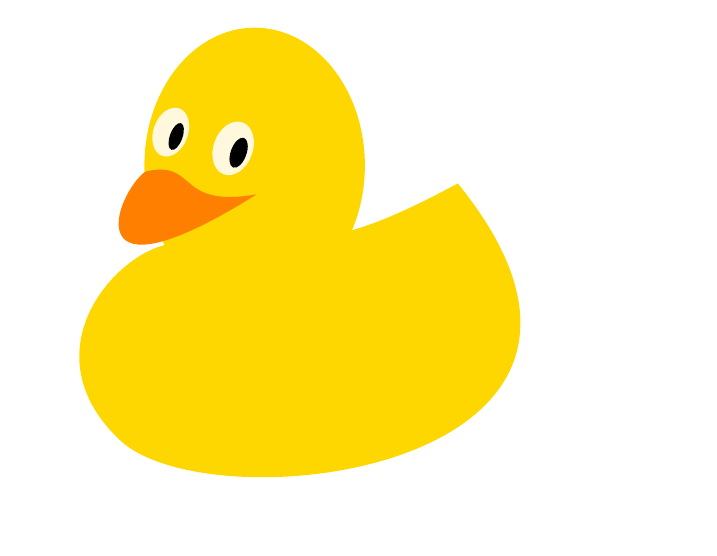
\begin{tikzpicture}[y=0.80pt, x=0.80pt, yscale=-1.000000, xscale=1.000000, inner sep=0pt, outer sep=0pt]
	\duck{Gold}
\end{tikzpicture}
%% blue duck
%\begin{tikzpicture}[y=0.80pt, x=0.80pt, yscale=-1.000000, xscale=1.000000, inner sep=0pt, outer sep=0pt]
%	\duck{SteelBlue}
%\end{tikzpicture}
%
%% alien duck
%\begin{tikzpicture}[y=0.80pt, x=0.80pt, yscale=-1.000000, xscale=1.000000, inner sep=0pt, outer sep=0pt]
%	\duck{Gold}
%	\addalien
%\end{tikzpicture}
%%
%% hat duck
%\begin{tikzpicture}[y=0.80pt, x=0.80pt, yscale=-1.000000, xscale=1.000000, inner sep=0pt, outer sep=0pt]
%	\duck{Gold}
%	\addhat{SaddleBrown}
%\end{tikzpicture}

\end{document}
